\documentclass{exam}
\usepackage[utf8]{inputenc}
\usepackage{lmodern}
\usepackage{microtype}

% \usepackage[parfill]{parskip}
\usepackage[dvipsnames]{xcolor}
\usepackage{amsmath}
\usepackage{amsfonts}
\usepackage{amsthm}
\usepackage{siunitx}
\DeclareSIUnit\year{yr}
\DeclareSIUnit\foot{ft}
\DeclareSIUnit\litre{\liter}

\usepackage{skull}

\usepackage{pgfplots}
\usepgfplotslibrary{polar}
\pgfplotsset{compat=1.11}
\usepgfplotslibrary{statistics}
\usepackage{graphicx}
\usepackage{sidecap}
\sidecaptionvpos{figure}{c}
\usepackage{float}
\usepackage{gensymb}
\usepackage{tkz-euclide}
\usetkzobj{all}
\usepackage{commath}
\usepackage{hyperref}
\usepackage{enumitem}
\usepackage{wasysym}
\usepackage{multicol}
\usepackage{mathtools}
\usepackage{tcolorbox}
\usepackage{tabularx}
\usepackage[version=4]{mhchem}
\usepackage{changepage}
\usepackage{listings}
\lstset{basicstyle=\ttfamily\linespread{0.8}\small}

\renewcommand*{\thefootnote}{\fnsymbol{footnote}}

\newtheorem*{thm}{Theorem}
\newtheorem*{iden}{Identity}
\newtheorem*{lemma}{Lemma}
\newtheorem{obs}{Observation}
\theoremstyle{definition}
\newtheorem*{defn}{Definition}
\newtheorem*{ex}{Example}
\newtheorem{con}{Construction}
\newtheorem*{alg}{Algorithm}

\newtheoremstyle{break}
  {\topsep}{\topsep}%
  {\itshape}{}%
  {\bfseries}{}%
  {\newline}{}%
\theoremstyle{break}
\newtheorem*{bthm}{Theorem}

% russian integral
\usepackage{scalerel}
\DeclareMathOperator*{\rint}{\scalerel*{\rotatebox{17}{$\!\int\!$}}{\int}}

% \DeclareMathOperator*{\rint}{\int}

\pgfplotsset{vasymptote/.style={
    before end axis/.append code={
        \draw[densely dashed] ({rel axis cs:0,0} -| {axis cs:#1,0})
        -- ({rel axis cs:0,1} -| {axis cs:#1,0});
    }
}}

% \pointsinrightmargin
\boxedpoints
\pointname{}

\newcommand{\questioA}{\question[\texttt{\textbf{\color{Cerulean} A}}]}
\newcommand{\questioM}{\question[\texttt{\textbf{\color{PineGreen} M}}]}
\newcommand{\questioE}{\question[\texttt{\textbf{\color{WildStrawberry} E}}]}
\newcommand{\questioS}{\question[\texttt{\textbf{\color{Goldenrod} S}}]}
\newcommand{\questioO}{\question[\texttt{\textbf{\color{BurntOrange} O}}]}

\newcommand{\parA}{\part[\texttt{\textbf{\color{Cerulean} A}}]}
\newcommand{\parM}{\part[\texttt{\textbf{\color{PineGreen} M}}]}
\newcommand{\parE}{\part[\texttt{\textbf{\color{WildStrawberry} E}}]}
\newcommand{\parS}{\part[\texttt{\textbf{\color{Goldenrod} S}}]}
\newcommand{\parO}{\part[\texttt{\textbf{\color{BurntOrange} O}}]}

\newcommand{\subparA}{\subpart[\texttt{\textbf{\color{Cerulean} A}}]}
\newcommand{\subparM}{\subpart[\texttt{\textbf{\color{PineGreen} M}}]}
\newcommand{\subparE}{\subpart[\texttt{\textbf{\color{WildStrawberry} E}}]}
\newcommand{\subparS}{\subpart[\texttt{\textbf{\color{Goldenrod} S}}]}
\newcommand{\subparO}{\subpart[\texttt{\textbf{\color{BurntOrange} O}}]}

\newcommand{\mainHeader}[2]{\section*{NCEA Level 2 Mathematics\\#1. #2}}
\newcommand{\mainHeaderHw}[2]{\section*{NCEA Level 2 Mathematics (Homework)\\#1. #2}}
\newcommand{\seealso}[1]{\begin{center}\emph{See also #1.}\end{center}}
\newcommand{\drills}[1]{\begin{center}\emph{Drill problems: #1.}\end{center}}
\newcommand{\basedon}[1]{\begin{center}\emph{Notes largely based on #1.}\end{center}}

\begin{document}

\mainHeaderDiff{7}{The Geometry of Functions}
\goals{To follow on from last week by using calculus to describe the geometry of the graph of a function.}
This week, we move on from approximating functions with straight lines to actually studying the geometry of the
curves themselves. Back in the homework on limits, I gave you the following definitions:

\begin{defn}\leavevmode
  \begin{enumerate}
    \item A function is \textbf{increasing} if its derivative is positive.
    \item A function is \textbf{decreasing} if its derivative is negative.
    \item A function is \textbf{concave down} if its derivative is decreasing.
    \item A function is \textbf{concave up} if its derivative is increasing.
    \item A function $ f $ is \textbf{continuous} at a point $ a $ if $ \lim_{x \to a} f(x) = f(a) $.
  \end{enumerate}
\end{defn}

\begin{exs}\leavevmode
  \begin{enumerate}
    \item The function $ x \mapsto x^2 $ is concave up everywhere, increasing for $ x > 0 $, and decreasing when $ x < 0 $.
    \item The function $ x \mapsto \sin x $ is concave down when $ (2n)\pi < x < (2n + 1)\pi $, and concave up when $ (2n + 1)\pi < x < (2n + 2)\pi $
          (for all integers $ n $).
          \begin{center}
            \fbox{\begin{tikzpicture}
              \begin{axis}[
                axis lines = center,
                ymax = 1.5, ymin = -1.5,
                xtick={-6.28, -4.7124, -3.14159, -1.5708, 1.5708, 3.14159, 4.7124, 6.28},
                xticklabels={$ -2\pi $, $ -\frac{3\pi}{2} $, $ -\pi $, $ -\frac{\pi}{2} $, $ \frac{\pi}{2} $, $ \pi $, $ \frac{3\pi}{2} $, $ 2\pi $},
                xlabel = $ x $,
                ylabel = $ y $
              ]
                \addplot[domain = -2*pi:2*pi, color = red, samples=100] {sin(deg(x))};
              \end{axis}
            \end{tikzpicture}}
          \end{center}
  \end{enumerate}
\end{exs}

We can tell if a function is increasing (getting larger) or decreasing (getting smaller) around a point by looking at the derivative
at that point. In order to look for concavity we must look at the derivative of the derivative (the second derivative). If
a function is concave up (curving up), the second derivative is positive; if a function is concave down at a point, then the second
derivative is negative. These facts are not ones which you should memorise, but ones which you should be able to reason about yourself
based on the graph of a function.

A point where a function changes from concave up to concave down (or vice versa) is known as an \textbf{inflection point}.

\begin{ex}
  The function $ x \mapsto x^3 $ has an inflection point at $ (0,0) $; to the left of this point, the function is concave
  down (the second derivative is negative) and to the right the function is concave up (the second derivative is positive).

  In general, functions of the form $ f(x) = x^n $ (for integer $ n \geq 0 $) have some fairly symmetric properties:
  \begin{itemize}
    \item If $ n $ is even, then $ y = f(x) $ is even around the $ x $-axis (i.e. $ f(-x) = f(x) $), has a minimum at $ (0,0) $, and
          tends to $ +\infty $ in both directions. (See the function graphed in blue in the diagram below.)
    \item If $ n $ is odd, then $ y = x^n $ is odd around the $ x $-axis (i.e. $ f(-x) = -f(x) $), has an inflection point at $ (0,0) $,
          and tends to $ -\infty $ towards the left and $ +\infty $ towards the right. (See the function graphed in red in the diagram below.)
  \end{itemize}

  \begin{center}
    \fbox{\begin{tikzpicture}
      \begin{axis}[
        axis lines = center,
        xlabel = $ x $,
        ylabel = {$ y $},
        ymin =
      ]
        \addplot[domain=-5:5, color=red, samples=200] {x^3};
        \addplot[domain=-10:10, color=blue, samples=200] {x^2};
      \end{axis}
    \end{tikzpicture}}
  \end{center}
\end{ex}

We call the value of the first derivative the \textit{slope} or \textit{gradient} of the function at a point; similarly,
the second derivative measures how "curvy" a function is and we call its value the \textit{concavity} of a function
at a point.

We also want to study continuity: a function is continuous, intuitively, if its graph can be drawn without picking a pen up off
the page. It is perhaps unfortunate that the concepts of continuity and differentiability are not the same. The details of this
are worked in the exercises.

\begin{ex}
  Consider the function defined by $ f(x) = x^4 - 2x^2 + 3 $. Find the intervals on which $ f $
  is increasing or decreasing, find the intervals of concavity, and find any inflection points.

  \textit{Solution.} We have $ f'(x) = 4x^3 - 4x $. This function is zero at $ x \in \{-1, 0, 1\} $, and so (since the function
  is a positive cubic) $ f $ will be decreasing when $ x < -1 $, increasing when $ -1 < x < 0 $, decreasing when $ 0 < x < 1 $,
  and increasing when $ 1 < x $. We also have $ f''(x) = 12x^2 - 4 $ and so $ f''(x) = 0 $ when $ x = \pm \frac{1}{\sqrt{3}} $.
  Hence the function is concave up when $ x < -\frac{1}{\sqrt{3}} $, concave down when $ \abs{x} < \frac{1}{\sqrt{3}} $, and concave
  up when $ x > \frac{1}{\sqrt{3}} $. The inflection points will be $ x = \pm{1}{\sqrt{3}} $.
  \begin{center}
    \fbox{\begin{tikzpicture}
      \begin{axis}[
        axis lines = center,
        xlabel = $ x $,
        ylabel = {$ y = f(x) $}
      ]
        \addplot[domain=-2:2, color=red, samples=200] {x^4 - 2*x^2 + 3};
      \end{axis}
    \end{tikzpicture}}
  \end{center}
\end{ex}

\clearpage
\subsection*{Questions}
\begin{questions}
  \questioA Find the second derivative of the following functions.
    \begin{parts}
      \part $ y = x^2 + x $
      \part $ f(x) = \sin x $
      \part $ g(x) = \cot(3x^2 + 5) $
      \part $ y = \frac{\sin mx}{x} $
      \part $ y = 4 \sin^2 x $
      \part $ y = \tan^2 (\sin \theta) $
      \part $ y = \tan \sqrt{1 - x} $
    \end{parts}
  \questioA Find the concavity of the function $ y = \frac{x^2 - 1}{x^2 + 1} $ at $ (0, -1) $.
  \questioM Find the intervals on which the following functions are increasing or decreasing, and
            find their intervals of concavity.
    \begin{parts}
      \part $ y = x^2 + 1 $
      \part $ y = 2x^3+ 3x^2 - 36x $
      \part $ G(x) = x - 4\sqrt{x} $
    \end{parts}
  \questioA The following function is known as the \textit{logistic curve} and is used for population modelling. Find the intervals of
            concavity, and label any inflection points.
            \begin{center}
              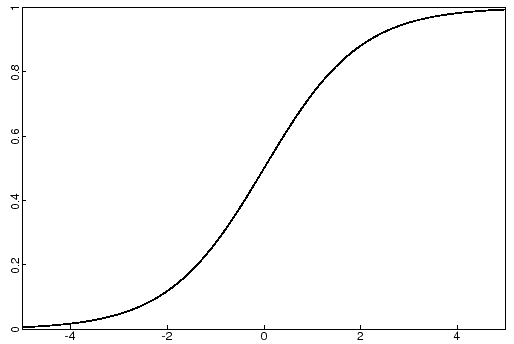
\includegraphics[width=0.4\textwidth]{logistic}
            \end{center}
  \questioM The graph of $ y = f(x) $ (where $ f $ is a continuous function) is concave up for all $ x < 0 $, concave down for $ x > 0 $, and decreasing everywhere.
    \begin{parts}
      \part Sketch the graph of $ y = f(x) $.
      \part What can you say about $ f'(x) $ and $ f''(x) $ for $ x < 0 $ and $ x > 0 $?
      \part What about $ x = 0 $?
    \end{parts}
  \questioE Find a value of $ k $ such that the function $ F $ is continuous at $ x = -3 $, where
            \begin{displaymath}
              F(x) =
              \begin{cases}
                \frac{x^2 - 9}{x+3} & \text{if } x \neq -3,\\
                k                   & \text{if } x = -3.
              \end{cases}
            \end{displaymath}
  \questioE Show whether or not the function $ g $ is continuous at the three points 2, 3, and 4, where
            \begin{displaymath}
              g(x) =
              \begin{cases}
                2x-x^2              & \text{if } 0 \leq 2,\\
                2-x                 & \text{if } 2 < x \leq 3,\\
                x-4                 & \text{if } 3 < x \leq 4,\\
                \pi                 & \text{if } x \geq 4.
              \end{cases}
            \end{displaymath}
  \questioE Find all values of $ \alpha $ such that $ \Phi $ is continuous everywhere, where
            \begin{displaymath}
              \Phi(x) =
              \begin{cases}
                x+1                 & \text{if } x \leq \alpha, \\
                x^2                 & \text{if } x > \alpha.
              \end{cases}
            \end{displaymath}
  \questioM Sketch a function satisfying the given criteria.
    \begin{parts}
      \part
        \begin{subparts}
          \subpart Vertical asymptote at $ x = 0 $,
          \subpart $ f'(x) > 0 $ if $ x < -2 $,
          \subpart $ f'(x) < 0 $ if $ x > -2 $ ($ x \neq 0 $),
          \subpart $ f''(x) < 0 $ if $ x < 0 $, $ f''(x) > 0 $ if $ x > 0 $.
        \end{subparts}
      \part
        \begin{subparts}
          \subpart $ f'(0) = f'(2) = f'(4) = 0 $,
          \subpart $ f'(x) > 0 $ if $ x < 0 $ or $ 2 < x < 4 $,
          \subpart $ f'(x) < 0 $ if $ 0 < x < 2 $ or $ x > 4 $,
          \subpart $ f''(x) > 0 $ if $ 1 < x < 3 $,
          \subpart $ f''(x) < 0 $ if $ x < 1 $ or $ x > 3 $.
        \end{subparts}
    \end{parts}
  \questioE A curve is defined by the function $ f(x) = e^{-(x-k)^2} $. Find, in terms of $ k $, the $ x$-ordinates for which $ f''(x) = 0 $.
  \questioS We will prove that differentiability of $ f $ at $ a $ implies continuity of $ f $ at $ a $; expand the following
            and use the limit laws to show that $ \lim_{x \to a} f(x) - f(a) = 0 $, carefully indicating where you use the existence
            of the derivative.
            \begin{displaymath}
              \left[\lim_{a \to x} f(x) - f(a)\right]\left[\lim_{a \to x} \frac{x - a}{x - a}\right]
            \end{displaymath}
  \questioE Give an example of a function which is continuous but not differentiable at some point.
  \questioS Scholarship 2010: Recall that the points of inflection of a curve are places where the second derivative
            changes sign. These are typically, \textbf{but not always}, points at which the second derivative is zero.

            Consider the curve $ y = \sqrt[3]{x} e^{-x^2} $.

            Write the second derivative in the form $ \od[2]{y}{x} = (ax^4 + bx^2 + x)e^{-x^2} x^{-5/3} $, and hence
            find the $ x$-ordinates of the points of inflection of the curve.
  \questioS Scholarship 2004: (You may wish to remind yourself how to perform long division of polynomials.) Consider the function
            \begin{displaymath}
              y = \frac{x^2}{1 + x^2},
            \end{displaymath}
            where $ -1 \leq x \leq 1 $. The gradient at the point $ x = 1 $ is $ \frac{1}{2} $.

            Hence show that there is a point with $ \frac{1}{4} \leq x \leq \frac{1}{2} $ where the gradient is also $ \frac{1}{2} $.
  \questioS Scholarship 2013: A function $ f $ is \textbf{even} if $ f(-x) = f(x) $ for all $ x $ in its domain, and \textbf{odd} if $ f(-x) = f(-x) $
            for all $ x $ in its domain.
    \begin{parts}
      \part Describe which polynomials are even, which are odd, and which are neither.
      \part Suppose that $ g $ is any even differentiable function defined for all real numbers (not necessarily a polynomial). Use the
            limit definition of the derivative to prove that $ g' $ is odd.
    \end{parts}
\end{questions}
\end{document}
